\section{Other Gradient Boosting Algorithms}

\begin{frame}
The last great feature of Gradient Boosting is that it generalizes easily to other loss functions.
\end{frame}
%
\begin{frame}
We will discuss two generalizations:

\begin{itemize}
  \item \textbf{Gradient Boosted Logistic Regression}: Minimizes the binomial deviance (logistic log likelihood) loss function.
  \item \textbf{AdaBoost}: Minimizes a custom classification loss.
\end{itemize}

It is important to say: \textit{There are many more possibilities}!
\end{frame}
%
\begin{frame}{Gradient Boosted Logistic Regression}
We want to generalize our boosting algorithm to also solve \textit{classification} problems. 

$$ y \in  \{0, 1\} $$

We want to estimate $ f(x) = Pr(y = 1 \mid x) $.
\end{frame}
%
\begin{frame}
For example, here is a complex classification problem

  \begin{figure}
    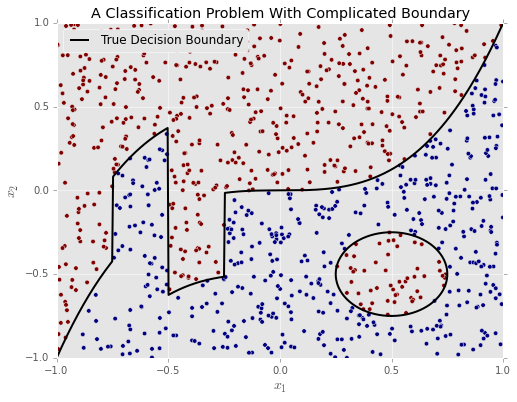
\includegraphics[scale=0.45]{classification-boundary-with-data}
  \end{figure}

\end{frame}
%
\begin{frame}
How would you solve this with standard logistic regression?

  \begin{figure}
    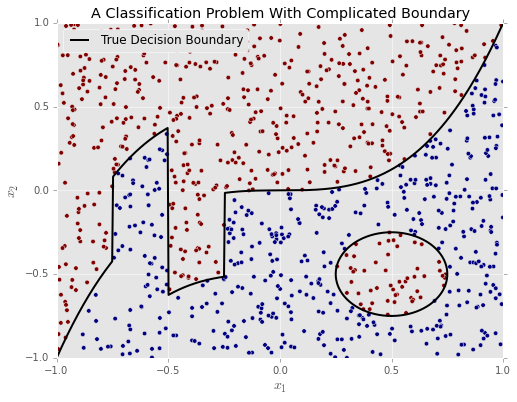
\includegraphics[scale=0.45]{classification-boundary-with-data}
  \end{figure}

\end{frame}
%
\begin{frame}
Gradient boosted logistic regression makes short work of it.

  \begin{figure}
    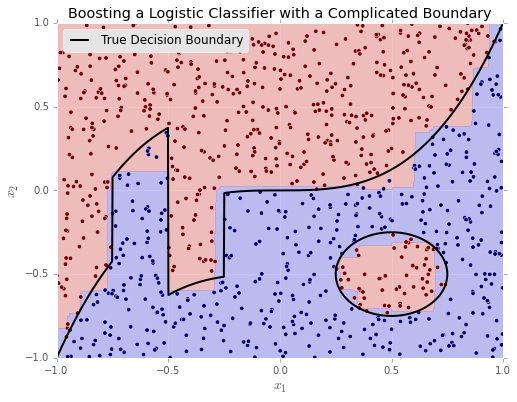
\includegraphics[scale=0.45]{classification-boundary-with-booster}
  \end{figure}

\end{frame}
%
\begin{frame}
Recall our friend logistic regression.

$$ \hat \beta = \argmin_{\beta} \sum_i \left( y_i \nu(\beta, x_i) - \log(1 + e^{\nu(\beta, x_i)}) \right) $$

Where $\nu(\beta, x_i) = \beta_0 + \beta_1 x_{i1} + \cdots + \beta_{M} x_{iM}$.\\~\\ 

The quantity $\nu$ is called the \textit{linear predictor}.\\~\\

In logistic regression it represents the \textit{log odds} of the outcome.
\end{frame}
%
\begin{frame}
Once we have solved for $\hat \beta$, we can make predictions using

$$p(x) = \frac{1}{1 + e^{-(\hat \beta_0 + \hat \beta_1 x_1 + \cdots + \hat \beta_M x_M)}}$$

The predictions can interpreted as \textit{the conditional probability that $y = 1$, given the values of $x$}.

$$ p(x) = Pr(y = 1 \mid x) $$
\end{frame}
%
\begin{frame}
The function we are minimizing in logistic regression is called the \textit{logistic loss}:

$$ L(f, y) = y f - \log(1 + e^{f}) $$

  \begin{figure}
    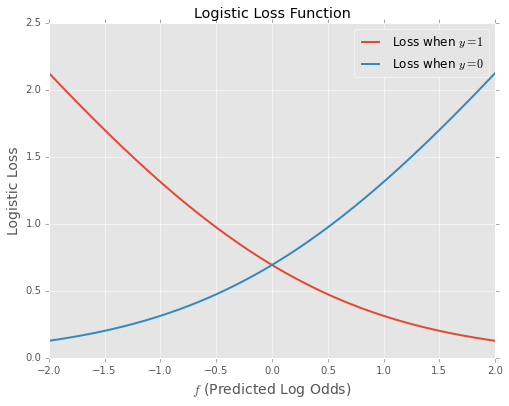
\includegraphics[scale=0.42]{loss-function-logistic}
  \end{figure}
  
\end{frame}
%
\begin{frame}
  \begin{center}
    \textbf{Logistic regression can be solved with gradient descent.}
  \end{center}
\end{frame}
%
\begin{frame}
\textbf{Gradient Boosted Logistic Regression}:\\~\\
Replace the linear predictor in logistic regression 

$$\nu(\beta, x) = \beta_0 + \beta_1 x_1 + \cdots + \beta_{M} x_M$$

With a sum of small regression trees

$$\nu(x) = T_0(x) + T_1(x) + \cdots + T_{\text{max}}(x)$$
\end{frame}
%
\begin{frame}
To fit a Gradient Boosted Logistic Regression, replace the least squares loss function

$$ L(f, y) = \frac{1}{2} \left(f - y \right)^2 $$

With the logistic loss

$$ L(f, y) = y f - \log(1 + e^f) $$

And then use the same gradient boosting technique.

\end{frame}
%
\begin{frame}
The gradient of the logistic loss is

\begin{align*}
\nabla_f L(f, y) &= \frac{\partial}{\partial f} \left( y f - \log(1 + e^f) \right) \\
&= y - \frac{e^f}{1 + e^f} \\
&= y - p(f)
\end{align*}

So we can interpret this method as "boosting to the residual probabilities".
\end{frame}
%

\begin{frame}
\textbf{Note:} There are some subtleties.  I've included the details in an appendix.
\end{frame}
%
\begin{frame}[fragile]
Gradient boosted logistic regression is implemented in sklearn as\\~\\

\begin{lstlisting}[language=python]
from sklearn.ensembles import GradientBoostingClassifier
model = GradientBoostingClassifier()
# Now y must be a np.array of 0 and 1's!
model.fit(X, y)
\end{lstlisting}
\end{frame}
%
\begin{frame}[fragile]
The options to \texttt{GradientBoostingClassifier} are the same as those to \texttt{GradientBoostingRegressor}\\~\\

\begin{lstlisting}[language=python]
GradientBoostingClassifier(loss='deviance',
                           n_estimators=100, 
                           learning_rate=0.1, 
                           max_depth=3,
                           subsample=1.0, 
                           min_samples_split=2, 
                           min_samples_leaf=1, 
                           min_weight_fraction_leaf=0.0,
                           ...)
\end{lstlisting}

And everything we said before generalizes.
\end{frame}
%
\begin{frame}[fragile]
To make predictions use \texttt{predict\_proba}\\~\\

\begin{lstlisting}[language=python]
model.predict_proba(X)
\end{lstlisting}

The \texttt{predict} method returns \textit{class labels} (by comparing the probability to $0.5$), making it much less useful.
\end{frame}
%
\begin{frame}[fragile]{Gradient Boosted AdaBoost}
By using the \texttt{'exponential'} loss, we get the Adaboost algorithm:

\begin{lstlisting}[language=python]
model = GradientBoostingClassifier(loss='exponential')
model.fit(X, y)
\end{lstlisting}

\end{frame}
%
\begin{frame}
The Adaboost algorithm uses labels $y \in \{-1, 1\}$ and minimizes the loss function

$$ L(f, y) = \exp( - y f) $$

  \begin{figure}
    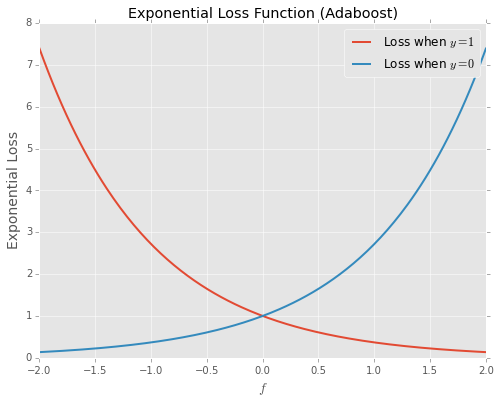
\includegraphics[scale=0.42]{loss-function-adaboost}
  \end{figure}

\end{frame}
%
\begin{frame}
The performance of Adaboost is generally comparable to that of gradient boosted logistic regression

  \begin{figure}
  
    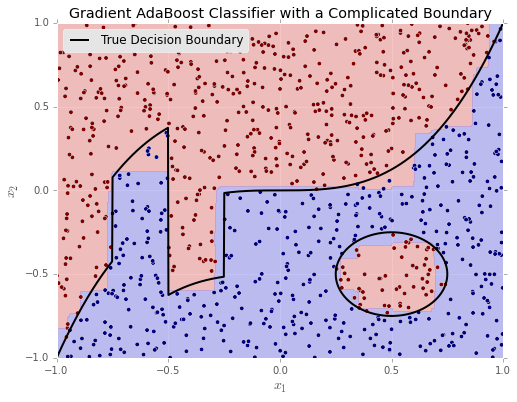
\includegraphics[scale=0.45]{classification-boundary-with-ada-gradient-booster}
  \end{figure}
  
\end{frame}
%
\begin{frame}
In fact, the classification boundaries are \textit{the same}

  \begin{columns}
    \column{.5\textwidth}
    \begin{figure}
      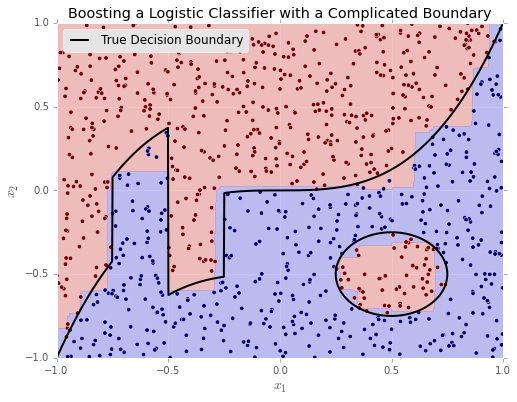
\includegraphics[scale=0.28]{classification-boundary-with-booster}
    \end{figure}
    \column{.5\textwidth}
    \begin{figure}
      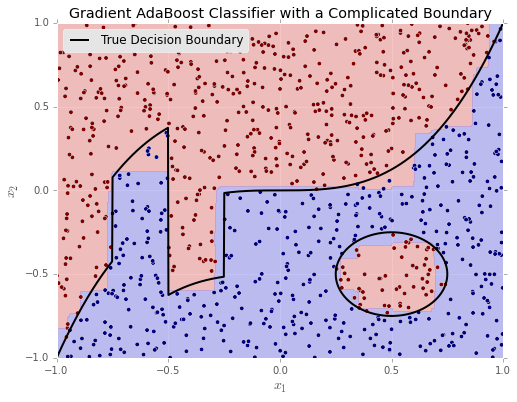
\includegraphics[scale=0.28]{classification-boundary-with-ada-gradient-booster}
    \end{figure}
  \end{columns}
  
\end{frame}
%
\begin{frame}
Gradient boosted logistic regression is less sensitive to outliers than Adaboost.  Can you see why?

  \begin{figure}
    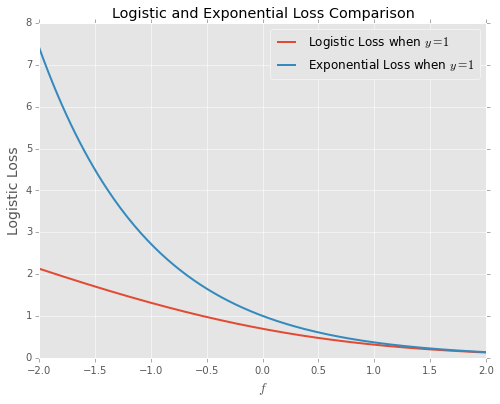
\includegraphics[scale=0.45]{loss-function-comparison}
  \end{figure}
  
\end{frame}
%
\begin{frame}[fragile]
The implementation of Adaboost as a gradient booster is a somewhat recent development.\\~\\

Originally (before the invention of gradient boosting), Adaboost was accomplished by a complicated sample re-weigting scheme.\\~\\
\end{frame}
%
\begin{frame}[fragile]
The traditional Adaboost is included in sklearn as \texttt{AdaBoostClassifier}\\~\\

\begin{lstlisting}[language=python]
model = AdaBoostClassifier()
model.fit(X, y)
\end{lstlisting}

Traditional Adaboost always uses trees of depth $1$ (often playfully called "stumps", so there is no \texttt{max\_depth} argument.
\end{frame}

%
\begin{frame}[fragile]
Traditional Adaboost is outclassed by gradient boosting, but retains historical and mathematical significance

  \begin{figure}
    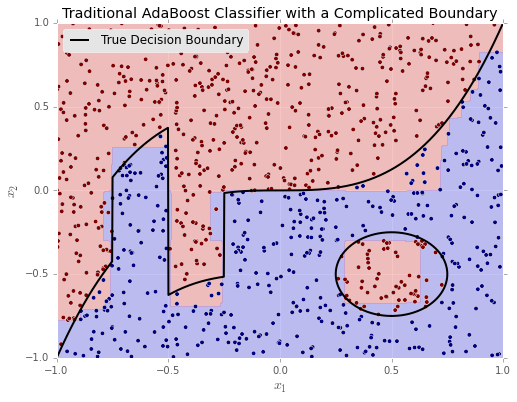
\includegraphics[scale=0.45]{classification-boundary-with-ada-booster}
  \end{figure}
 
\end{frame}
%
\begin{frame}{A Final Comparison of Classification Algorithms}

  \begin{figure}
    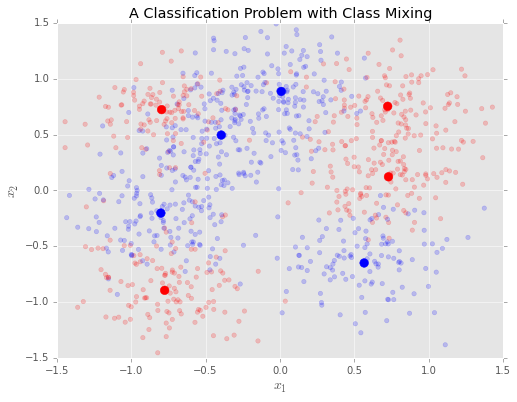
\includegraphics[scale=0.5]{classification-mixed}
  \end{figure}

\end{frame}
%
\begin{frame}

  \begin{figure}
    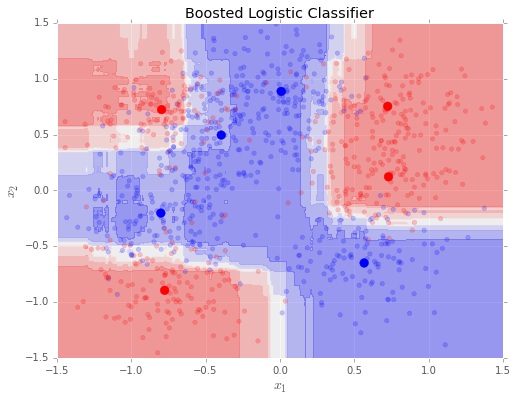
\includegraphics[scale=0.5]{classification-mixed-logistic-boosting}
  \end{figure}
  
\end{frame}
%
\begin{frame}

  \begin{figure}
    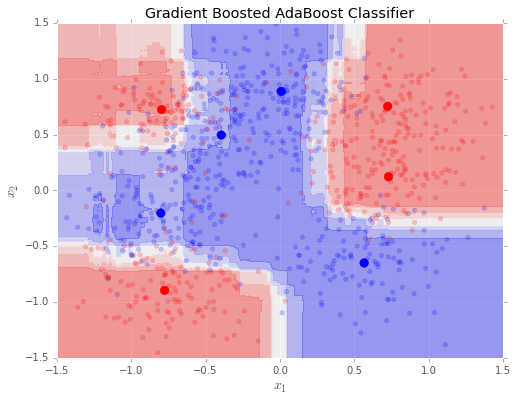
\includegraphics[scale=0.5]{classification-mixed-ada-gradient-boosting}
  \end{figure}
  
\end{frame}
%
\begin{frame}

  \begin{figure}
    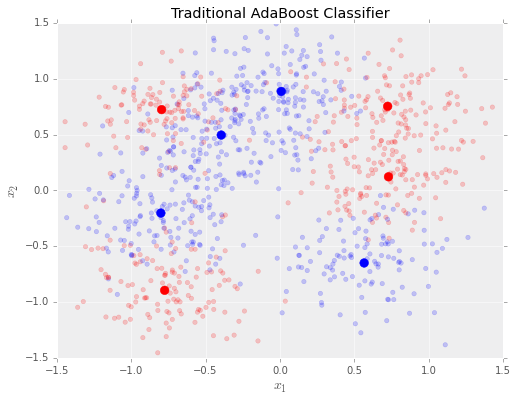
\includegraphics[scale=0.5]{classification-mixed-ada-traditional-boosting}
  \end{figure}
  
\end{frame}
%
\begin{frame}

  \begin{figure}
    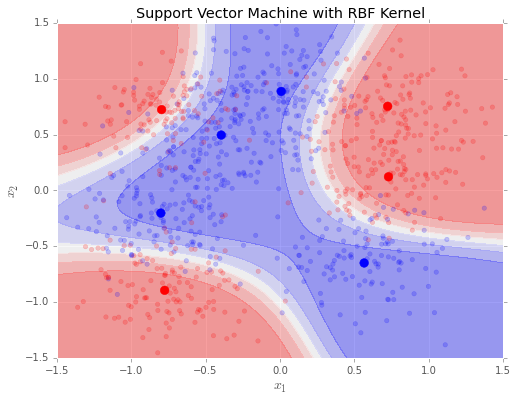
\includegraphics[scale=0.5]{classification-mixed-svm}
  \end{figure}
  
\end{frame}
%
\begin{frame}

  \begin{figure}
    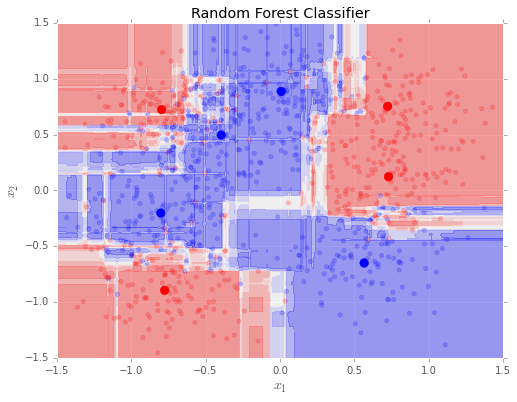
\includegraphics[scale=0.5]{classification-mixed-random-forest}
  \end{figure}
  
\end{frame}